\documentclass{article}

% Set page size and margins
% Replace `letterpaper' with `a4paper' for UK/EU standard size
\usepackage[letterpaper,top=2cm,bottom=2cm,left=3cm,right=3cm,marginparwidth=1.75cm]{geometry}

\usepackage{amsmath}
\usepackage{graphicx}
\usepackage[colorlinks=true, allcolors=blue]{hyperref}
\usepackage[utf8]{inputenc}
\usepackage[russian]{babel}

\title{СВТ, Домашнее задание №2}
\author{Агеев Николай, 303 группа}

\begin{document}
\maketitle

\section{Описание задачи}

Требуется численно решить двумерную краевую задачу Дирихле для уравнения Лапласа:
$$
\begin{cases}
-\Delta u(x, y) = f(x, y), \quad (x, y) \in \Omega = (0; 1)\times(0; 1) \\
u\vert_{\partial \Omega} = g
\end{cases}
$$

Протестировать программу требуется на функции $u(x) = \sin (5x) \sin (5y)$. Таким образом, правая часть в системе равна $f(x, y) = -\Delta u(x, y) = 50 \sin (5x) \sin (5y)$.

\section{Описание метода}

\subsection{Аппроксимация уравнения Лапласа}

Решение краевой задачи нужно искать с помощью метода конечных разностей. 
В квадрате $[0; 1]\times[0; 1]$ вводится равномерная сетка $\{x_{ij}\}_{i, j = 0}^N$, где $x_{ij} = (ih, jh)$, $h = 1 / N$ - шаг сетки. Вводятся дискретные неизвестные $y_{ij} = u(x_{ij}), \ i,j = 0, 1, 2, ... , N$. В каждой точке $x_{ij}, \ i, j = 1, ... , N - 1$ лапласиан функции приближается формулой конечных разностей по пяти точкам:
$$
\Delta u(x_{i,j}) \approx \frac{y_{i - 1, j} - 2y_{i, j} + y_{i + 1, j}}{h^2} + \frac{y_{i, j - 1} - 2y_{i, j} + y_{i, j + 1}}{h^2}
$$
Таким образом, получается дискретная аппроксимация уравнения:
$$
-\frac{y_{i - 1, j} - 2y_{i, j} + y_{i + 1, j}}{h^2} - \frac{y_{i, j - 1} - 2y_{i, j} + y_{i, j + 1}}{h^2} = f(x_{i, j})
\Longrightarrow
$$
$$\frac{1}{h^2} \left ( 4y_{i,j} - y_{i - 1, j} - y_{i+1, j} - y_{i, j-1} - y_{i, j+1}\right ) = f(x_{i,j})$$

\subsection{Решение системы}

Так как для сетки с числом разбиений $N$ количество неизвестных равно $(N - 1)^2$, матрица системы $Ay = b$ будет иметь порядок $(N - 1)^2$. В каждой строке матрицы $A$ будет не более 5 ненулевых элементов.
С учётом граничных условий матрица для дискретного решения принимает вид
$$\frac{1}{h^2}Ay = b, \ \ A = \Vert a_{r,c} \Vert_{r, c = 1}^{(N-1)^2}$$
Обозначим $a_{(i, j), (k, l)} = a_{(i-1)(N-1)+j, (k-1)(N-1) + l}$, где $i, j, k, l = 1, ... , N-1$ - коеффициент при $y_{k, l}$ в шаблоне для приближения $-\Delta u(x_{i, j})$.
Тогда для всех $i, j = 1, ... , N-1$:
\begin{itemize}
  \item $a_{(i, j), (i, j)} = 4$
  \item если $i \ge 2$, то $a_{(i, j), (i - 1, j)} = -1$
  \item если $i \le N - 1$, то $a_{(i, j), (i + 1, j)} = -1$
  \item если $j \ge 2$, то $a_{(i, j), (i, j - 1)} = -1$
  \item если $i \le N - 1$, то $a_{(i, j), (i, j + 1)} = -1$
\end{itemize}

Аналогично обозначим $b_{(i, j)} = b_{(i - 1)(N-1) + j}$, где $i, j = 1, ... , N-1$ - требуемое значение $-\Delta u(x_{i, j})$ с учётом граничных условий.
Тогда для всех $i, j = 1, ... , N-1$:

$b_{(i, j)} = f(ih, jh) + ...$
\begin{itemize}
  \item $+ \frac{g(0, jh)}{h^2}$, если $i = 1$
  \item $+ \frac{g(1, jh)}{h^2}$, если $i = N-1$
  \item $+ \frac{g(ih, 0)}{h^2}$, если $j = 0$
  \item $+ \frac{g(ih, 1)}{h^2}$, если $j = N-1$
\end{itemize}

Данная система решается методом BiCGStab с предобуславливателем ILU2 при помощи функций из пакета INMOST.

\section{Результаты}

На построенном графике можно увидеть зависимость C-нормы и дискретной L2-нормы ошибки решения от числа отрезков сетки $N$. Относительная и абсолютная точности в методе были установлены равными $10^{-12}$, параметр \textit{drop\_tolerance} был установлен равным $0.005$.

\begin{figure}[!hq]
    \centering
    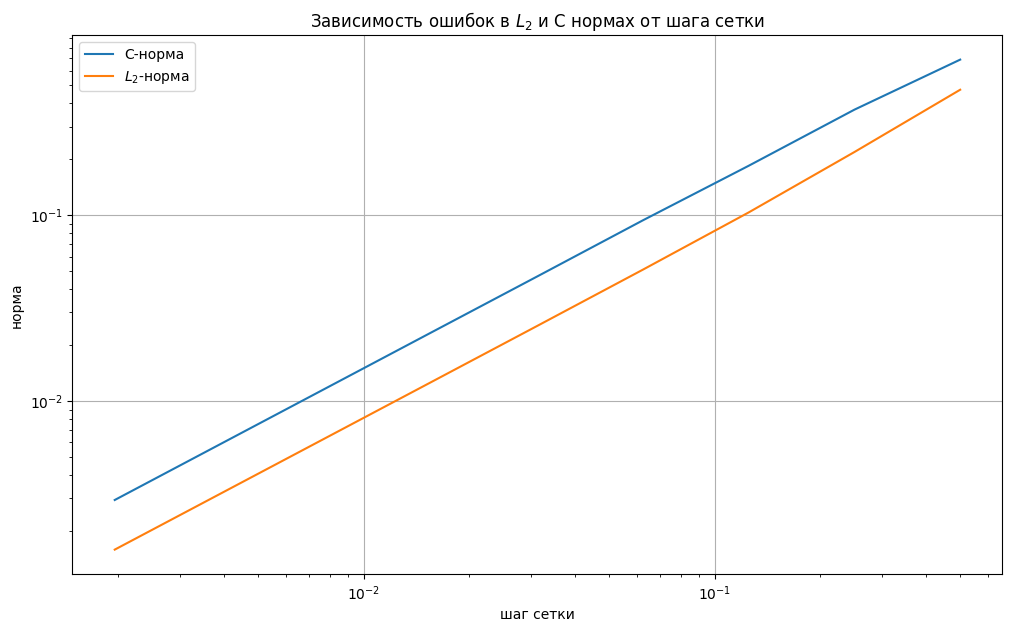
\includegraphics[width=1\linewidth]{error_norm_graph.png}
    \caption{Зависимость C-нормы и дискретной L2-нормы ошибки решения от шага сетки $h = \frac{1}{N}$}
    \label{fig:graph1}
\end{figure}

На следующих двух графиках изображена зависимость числа итераций, времени, затраченного на итерации и общего времени решения задачи от размера сетки $N$. 

\begin{figure}[!hq]
    \centering
    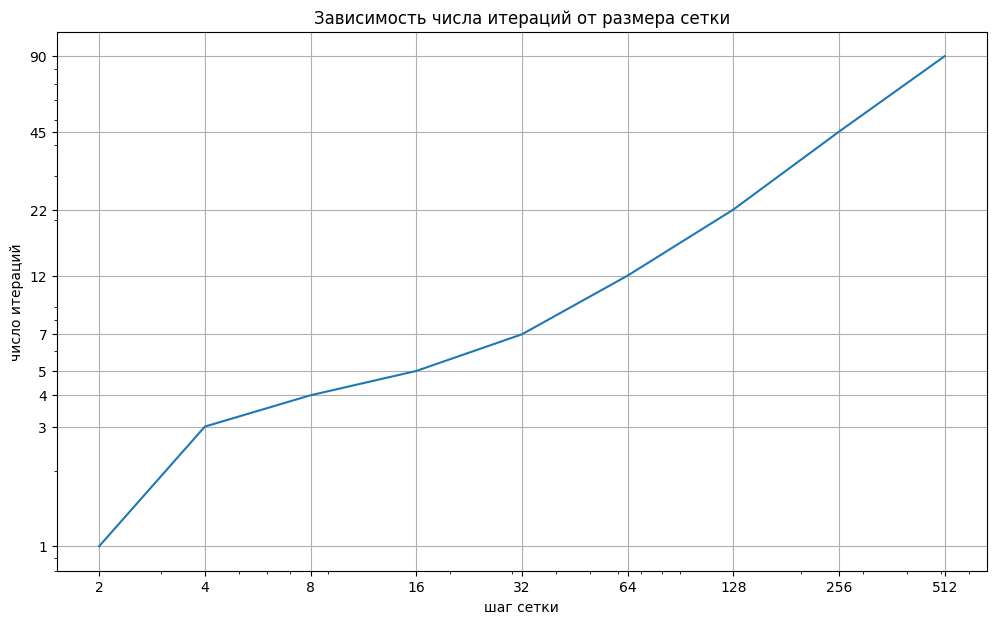
\includegraphics[width=1\linewidth]{iters_graph.png}
    \caption{Зависимость числа итераций от $N$}
    \label{fig:enter-label}
\end{figure}

\begin{figure}
    \centering
    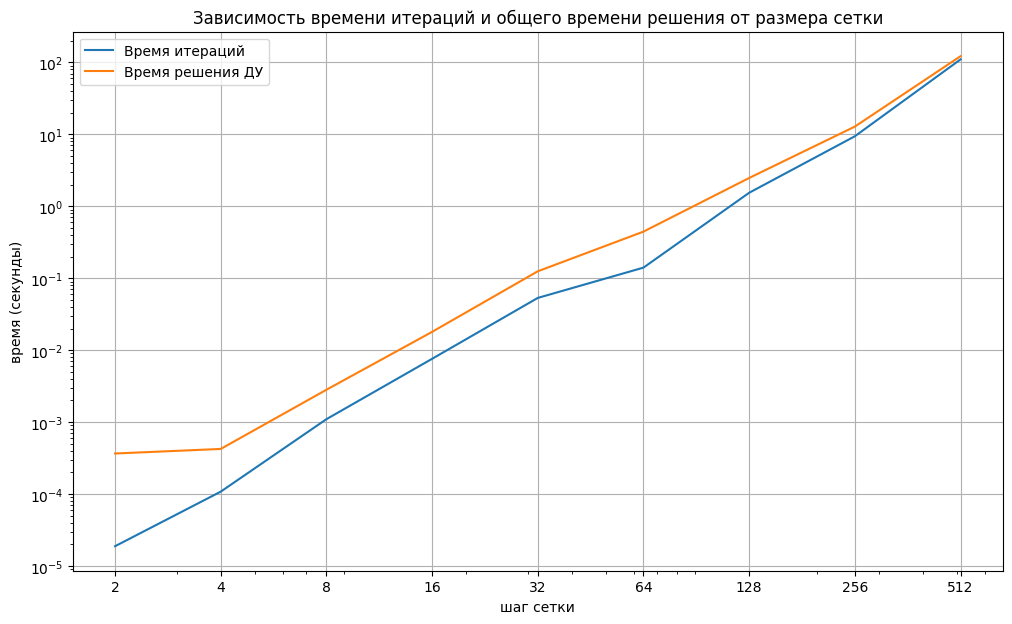
\includegraphics[width=1\linewidth]{time_graph.png}
    \caption{Зависимость времени итераций и общего времени решения задачи от $N$}
    \label{fig:graph3}
\end{figure}

\newpage

\begin{table}[]
\begin{tabular}{|l|l|l|l|l|l|}
\hline
N   & Число итераций & Время итераций & Время решения ДУ & L2-норма ошибки & С-норма ошибки \\ \hline
2   & 1              & 1.88351e-05    & 0.000366183      & 0.474164        & 0.688596       \\ \hline
4   & 3              & 0.000108004    & 0.000423785      & 0.219235        & 0.370556       \\ \hline
8   & 4              & 0.00109816     & 0.00281569       & 0.103753        & 0.184964       \\ \hline
16  & 5              & 0.0075829      & 0.0179637        & 0.0510823       & 0.0941381      \\ \hline
32  & 7              & 0.0532348      & 0.124809         & 0.0254388       & 0.0469567      \\ \hline
64  & 12             & 0.140356       & 0.444268         & 0.0127065       & 0.0234937      \\ \hline
128 & 22             & 1.54003        & 2.47284          & 0.00635162      & 0.0117459      \\ \hline
256 & 45             & 9.39308        & 12.8064          & 0.00317561      & 0.00587354     \\ \hline
512 & 90             & 109.899        & 121.808          & 0.00158776      & 0.00293672     \\ \hline
\end{tabular}
\caption{Зависимость C-нормы и дискретной L2-нормы ошибки решения от $N$}
\label{tab:table}
\end{table}

Из графика и таблицы видно, что обе нормы ошибки решения уменьшаются с уменьшением шага сетки.

\section{Выводы}

Написаны функции для численного решения двумерного уравнения Лапласа, протестированы на функции $u(x, y) = \sin (5x) \cos(5y)$, построены графики норм ошибок, числа итераций и времени и приведена таблица с результатами экспериментов.

\end{document}